%%%%%%%%%%%%%%%%%%%%%%%%%%%%%%%%%%%%%%%%%
% Beamer Presentation
% LaTeX Template
% Version 1.0 (10/11/12)
%
% This template has been downloaded from:
% http://www.LaTeXTemplates.com
%
% License:
% CC BY-NC-SA 3.0 (http://creativecommons.org/licenses/by-nc-sa/3.0/)
%
%%%%%%%%%%%%%%%%%%%%%%%%%%%%%%%%%%%%%%%%%

%----------------------------------------------------------------------------------------
%	PACKAGES AND THEMES
%----------------------------------------------------------------------------------------

\documentclass{beamer}

\mode<presentation> {

% The Beamer class comes with a number of default slide themes
% which change the colors and layouts of slides. Below this is a list
% of all the themes, uncomment each in turn to see what they look like.
\usepackage{vntex}
%\usetheme{default}
%\usetheme{AnnArbor}
%\usetheme{Antibes}
%\usetheme{Bergen}
%\usetheme{Berkeley}
%\usetheme{Berlin}
%\usetheme{Boadilla}
%\usetheme{CambridgeUS}
%\usetheme{Copenhagen}
%\usetheme{Darmstadt}
%\usetheme{Dresden}
%\usetheme{Frankfurt}
%\usetheme{Goettingen}
%\usetheme{Hannover}
%\usetheme{Ilmenau}
%\usetheme{JuanLesPins}
%\usetheme{Luebeck}
\usetheme{Madrid}
%\usetheme{Malmoe}
%\usetheme{Marburg}
%\usetheme{Montpellier}
%\usetheme{PaloAlto}
%\usetheme{Pittsburgh}
%\usetheme{Rochester}
%\usetheme{Singapore}
%\usetheme{Szeged}
%\usetheme{Warsaw}

% As well as themes, the Beamer class has a number of color themes
% for any slide theme. Uncomment each of these in turn to see how it
% changes the colors of your current slide theme.

%\usecolortheme{albatross}
%\usecolortheme{beaver}
%\usecolortheme{beetle}
%\usecolortheme{crane}
%\usecolortheme{dolphin}
%\usecolortheme{dove}
%\usecolortheme{fly}
%\usecolortheme{lily}
%\usecolortheme{orchid}
%\usecolortheme{rose}
%\usecolortheme{seagull}
%\usecolortheme{seahorse}
%\usecolortheme{whale}
%\usecolortheme{wolverine}

%\setbeamertemplate{footline} % To remove the footer line in all slides uncomment this line
%\setbeamertemplate{footline}[page number] % To replace the footer line in all slides with a simple slide count uncomment this line

%\setbeamertemplate{navigation symbols}{} % To remove the navigation symbols from the bottom of all slides uncomment this line
}

\usepackage{graphicx} % Allows including images
\usepackage{booktabs} % Allows the use of \toprule, \midrule and \bottomrule in tables
\usepackage[sorting=none,backend=biber]{biblatex}
% \addbibresource{rs_test.bib}
\addbibresource{rs1.bib}

\usepackage[utf8]{inputenc}

% \def\sectionname{\translate{Section}}
% \setbeamertemplate{section page}
% {
%   \begin{centering}
%     \vskip1em\par

%     \vspace{3cm}
% \begin{beamercolorbox}[sep=4pt,center]{part title}
%   \usebeamerfont{section title}\insertsection\par
% \end{beamercolorbox}
%   \end{centering}
% }

% \setbeamertemplate{section page2}
% {\tableofcontents[currentsection, sectionstyle=show/hide, subsectionstyle=show/show/hide]}

% \def\sectionpage{\usebeamertemplate*{section page}}
% \def\sectionpageBis{\usebeamertemplate*{section page2}}

% \AtBeginSection{ 
% \begin{frame}
%         \frametitle{Mục lục}
%         \tableofcontents[currentsection]
%     \end{frame}}
% \AtBeginSubsection[]
% {
%     \begin{frame}
%         \frametitle{Mục lục}
%         \tableofcontents[currentsection,currentsubsection]
%     \end{frame}
% }

\setbeamertemplate{footline}
{%
  \leavevmode%
  \hbox{%
  \begin{beamercolorbox}[wd=.333333\paperwidth,ht=2.25ex,dp=1ex,center]{author in head/foot}%
    \usebeamerfont{title in head/foot}\insertshorttitle
  \end{beamercolorbox}%
  \begin{beamercolorbox}[wd=.333333\paperwidth,ht=2.25ex,dp=1ex,center]{title in head/foot}%
    \usebeamerfont{title in head/foot}\insertsectionhead
  \end{beamercolorbox}%
  \begin{beamercolorbox}[wd=.333333\paperwidth,ht=2.25ex,dp=1ex,leftskip=2ex,rightskip=2ex,sep=0pt]{date in head/foot}%
    \hfill%
    \usebeamerfont{date in head/foot}%
    \insertshortdate{}%
    \hfill%
    \usebeamercolor[fg]{page number in head/foot}%
    \usebeamerfont{page number in head/foot}%
    \usebeamertemplate{page number in head/foot}%
  \end{beamercolorbox}}%
  \vskip0pt%
}
\setbeamertemplate{caption}[numbered]
\numberwithin{figure}{section}
\numberwithin{table}{section}




%----------------------------------------------------------------------------------------
%	TITLE PAGE
%----------------------------------------------------------------------------------------

\title[Luận văn thạc sĩ]{TỔNG HỢP GIỌNG NÓI SỬ DỤNG HỌC SÂU } % The short title appears at the bottom of every slide, the full title is only on the title page

\author{Hồ Minh Hoàng} % Your name
\institute[HCMUT] % Your institution as it will appear on the bottom of every slide, may be shorthand to save space
{
% University of California \\ % Your institution for the title page
% \medskip
\textit{Giảng viên hướng dẫn} \\
PGS.TS. Quản Thành Thơ \\
\medskip
\medskip
\medskip
Đại học Quốc gia Thành phố Hồ Chí Minh \\
Trường Đại học Bách Khoa \\
}


\date{\today} % Date, can be changed to a custom date
\begin{document}

\begin{frame}
\titlepage % Print the title page as the first slide
\end{frame}

\begin{frame}
\frametitle{Mục lục} % Table of contents slide, comment this block out to remove it
\tableofcontents % Throughout your presentation, if you choose to use \section{} and \subsection{} commands, these will automatically be printed on this slide as an overview of your presentation
\end{frame}


%----------------------------------------------------------------------------------------
%	PRESENTATION SLIDES
%----------------------------------------------------------------------------------------
%------------------------------------------------
\section{Giới thiệu}
{
    \begin{frame}
        \frametitle{Mục lục}
        \tableofcontents[currentsection]
    \end{frame}
}
%------------------------------------------------


% \subsection{Subsection Example} % A subsection can be created just before a set of slides with a common theme to further break down your presentation into chunks
\subsection{Giới thiệu đề tài}
{
    \begin{frame}
        \frametitle{Mục lục}
        \tableofcontents[currentsection, currentsubsection]
    \end{frame}
}
\begin{frame}
\frametitle{Giới thiệu về bài toán tổng hợp giọng nói}
\begin{figure}
    \centering
    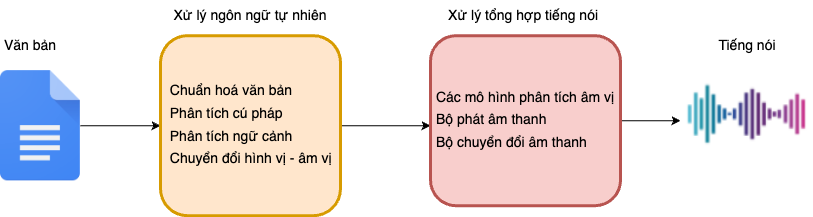
\includegraphics[scale=0.4]{image/tts-abs.png}
    \caption{Quá trình xử lý tổng hợp giọng nói từ văn bản}
\end{figure}


\end{frame}

%------------------------------------------------
%------------------------------------------------
\begin{frame}
\frametitle{Giới thiệu về đề tài}
\begin{itemize}
    \item [--] Các mô hình tổng hợp giọng nói hiện nay chủ yếu cho tiếng Anh và tiếng Trung \cite{survey}
    \pause
    \item [--] Người Bahnar là một dân tộc thiểu số ở Việt Nam được nhà nhà nước tìm cách để giữ gìn bản sắc, tiếng nói và lưu giữ các văn bản bằng tiếng Bahnar \footnote{\href{https://dangcongsan.vn/tu-tuong-van-hoa/bao-ton-van-hoa-truyen-thong-dan-toc-jrai-va-bahnar-367994.html}{Bảo tồn văn hóa truyền thống dân tộc J’rai và Bahnar}}
    \pause
    \item[$\rightarrow$] Việc có hệ thống dịch và tổng hợp giọng nói là cần thiết cho quá trình giữ gìn này 
\end{itemize}


\end{frame}

%------------------------------------------------
%------------------------------------------------

% \subsection{Subsection Example} % A subsection can be created just before a set of slides with a common theme to further break down your presentation into chunks
 \subsection{Mục tiêu đề tài}
 {
    \begin{frame}
        \frametitle{Mục lục}
        \tableofcontents[currentsection, currentsubsection]
    \end{frame}
}
\begin{frame}
\frametitle{Mục tiêu đề tài}
\begin{itemize}
    \item[--] Xây dựng, đề xuất mô hình chuyển đổi văn bản thành giọng nói cho tiếng Bahnar 

    \item[--] Tìm hiểu về các mô hình tổng hợp giọng nói, các công trình liên quan, các phương pháp giải quyết bài toán, ưu và nhược điểm của các phương pháp, đặc biệt là phương pháp sử dụng các mô hình học sâu. 

    \item[--] Thu thập tập dữ liệu thực tế và thực hiện xử lý dữ liệu để cho quá trình huấn luyện và đánh giá cho mô hình đề xuất.

    \item[--] Thực nghiệm, đánh giá kết quả của các mô hình đề xuất trên các tập dữ liệu đã được xử lý trước đó.

    \item[--] Chỉ ra những hạn chế và vấn đề tồn đọng, đề xuất các giải pháp cải tiến và mở rộng của bài toán trong tương lai.
\end{itemize}

\end{frame}

%------------------------------------------------

%------------------------------------------------
%------------------------------------------------


% \subsection{Subsection Example} % A subsection can be created just before a set of slides with a common theme to further break down your presentation into chunks
\subsection{Giới hạn đề tài}
{
    \begin{frame}
        \frametitle{Mục lục}
        \tableofcontents[currentsection, currentsubsection]
    \end{frame}
}
\begin{frame}
\frametitle{Giới hạn đề tài}
\begin{itemize}
    \item[--] Đề tài tập trung chủ yếu vào việc tổng hợp giọng nói.
    \item[--] Tập dữ liệu được sử dụng là tập tiếng dân tộc thiểu số Bahnar
    \item[--] Tìm hiểu các phương pháp và đưa ra đề xuất cho bài toán.
    \item[--] Xây dựng được mô hình có thể tổng hợp tiếng Bahnar với độ chính xác, có giọng đọc tự nhiên

\end{itemize}
\end{frame}

%------------------------------------------------

%------------------------------------------------


%------------------------------------------------

%------------------------------------------------
\section{Các nghiên cứu liên quan}
{
    \begin{frame}
        \frametitle{Mục lục}
        \tableofcontents[currentsection]
    \end{frame}
}
%------------------------------------------------
%------------------------------------------------


% \subsection{Subsection Example} % A subsection can be created just before a set of slides with a common theme to further break down your presentation into chunks
\subsection{Các phương pháp chuyển văn bản thành giọng nói}
{
    \begin{frame}
        \frametitle{Mục lục}
        \tableofcontents[currentsection, currentsubsection]
    \end{frame}
}
\begin{frame}
\frametitle{Các phương pháp chuyển văn bản thành giọng nói}
\begin{figure}
    \centering
    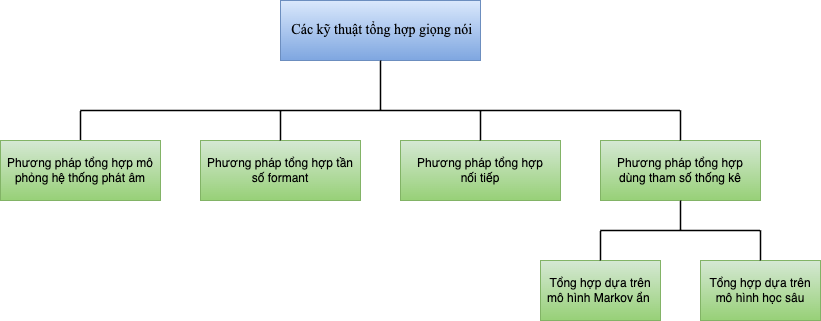
\includegraphics[scale=0.4]{image/tts-tax.png}
    \caption{Các hướng tiếp cận cho bài toán tổng hợp giọng nói}
\end{figure}
\end{frame}

%------------------------------------------------


\begin{frame}
\frametitle{Các phương pháp truyền thống}
\begin{itemize}
    \item Phương pháp tổng hợp mô phỏng hệ thống phát âm (Articulatory synthesis)
    \pause
    \item Phương pháp tổng hợp tần số formant (Formant synthesis)
    \begin{figure}
        \centering
        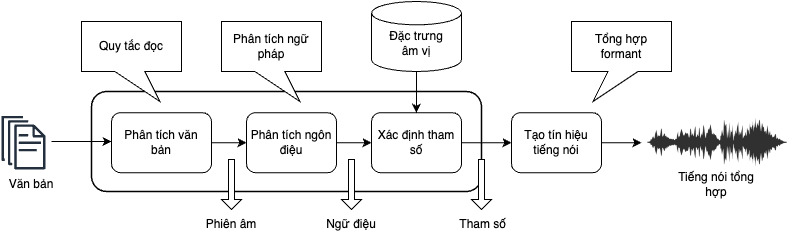
\includegraphics[scale=0.4]{image/formant.png}
        \caption{Phương pháp tổng hợp hình thái}
    \end{figure}
\end{itemize}
\end{frame}

\begin{frame}
\frametitle{Các phương pháp truyền thống}
\begin{itemize}
    \item Phương pháp tổng hợp mô phỏng hệ thống phát âm (Articulatory synthesis)
    \item Phương pháp tổng hợp tần số formant (Formant synthesis)
    \item Phương pháp tổng hợp nối tiếp (Concatenative synthesis)
    \begin{figure}
        \centering
        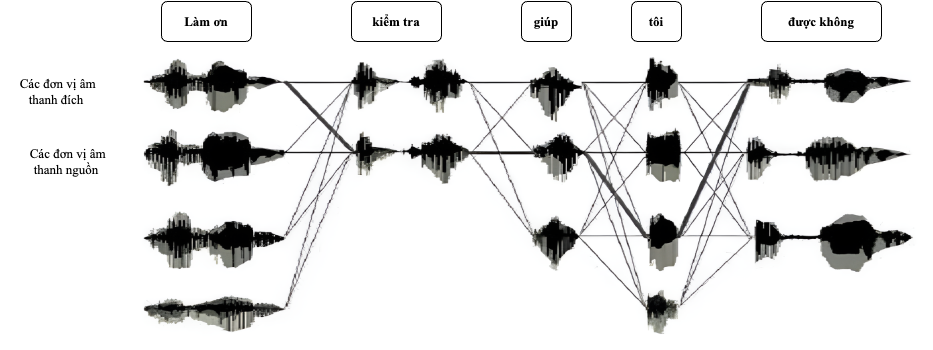
\includegraphics[scale=0.3]{image/concatenative.png}
        \caption{Phương pháp tổng hợp nối tiếp}
    \end{figure}
\end{itemize}
\end{frame}
%------------------------------------------------

%------------------------------------------------

\begin{frame}
\frametitle{Phương pháp tổng hợp tham số thống kê}
Phương pháp tổng hợp tham số thống kê (Statistical Parametric Speech Synthesis) gồm các nhánh
\begin{itemize}
    \item HMM-based Synthesis (HMM-based TTS)
    \pause
    \item Deep Learning-based Synthesis
\end{itemize}
\end{frame}
\begin{frame}
\frametitle{Các thành phần chính của mô hình tổng hợp giọng nói sử dụng học sâu}
Mô hình tổng hợp giọng nói sử dụng học sâu \cite{survey} gồm các thành phần chính như sau
\begin{figure}
    \centering
    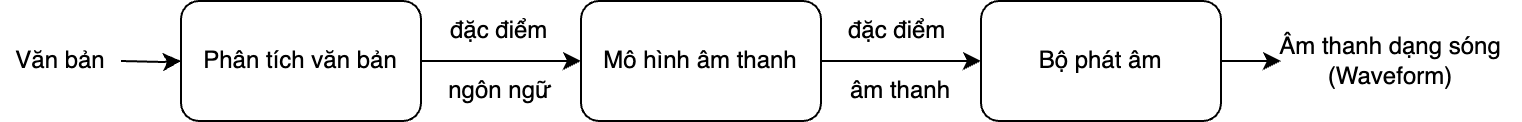
\includegraphics[scale=0.2]{image/tts-component.png}
    \caption{Kiến trúc mô hình TTS sử dụng học sâu}
\end{figure}
\end{frame}

%------------------------------------------------

%------------------------------------------------

\subsection{Các phương pháp chuyển đổi giọng nói}
{
    \begin{frame}
        \frametitle{Mục lục}
        \tableofcontents[currentsection, currentsubsection]
    \end{frame}
}
\begin{frame}
\frametitle{Các phương pháp chuyển đổi giọng nói}
Chuyển đổi giọng nói (VC) là một kỹ thuật chuyển đổi nhận dạng giọng nói của người nói này sang giọng nói khác trong khi vẫn giữ được nội dung ngôn ngữ \cite{survey_vc}. VC hiện tại chủ yếu dựa trên các mô hình học sâu. Dựa vào tập dự liệu huấn luyện đầu vào có thể chia thành 2 loại:
\begin{itemize}
    \item Parallel VC
    \item Non-parallel VC
\end{itemize}
\end{frame}

%------------------------------------------------

%------------------------------------------------
\section{Mô hình đề xuất}
{
    \begin{frame}
        \frametitle{Mục lục}
        \tableofcontents[currentsection]
    \end{frame}
}% Sections can be created in order to organize your presentation into discrete blocks, all sections and subsections are automatically printed in the table of contents as an overview of the talk
%------------------------------------------------
\subsection{Hệ thống ngữ âm tiếng Bahnar}
{
    \begin{frame}
        \frametitle{Mục lục}
        \tableofcontents[currentsection, currentsubsection]
    \end{frame}
}
\begin{frame}
\frametitle{Hệ thống ngữ âm tiếng Bahnar}
Tiếng Bahnaric thể hiện những đặc điểm độc đáo ngăn cản việc sử dụng các mô-đun phân tích cú pháp được thiết kế cho các ngôn ngữ khác
\begin{figure}
    \centering
    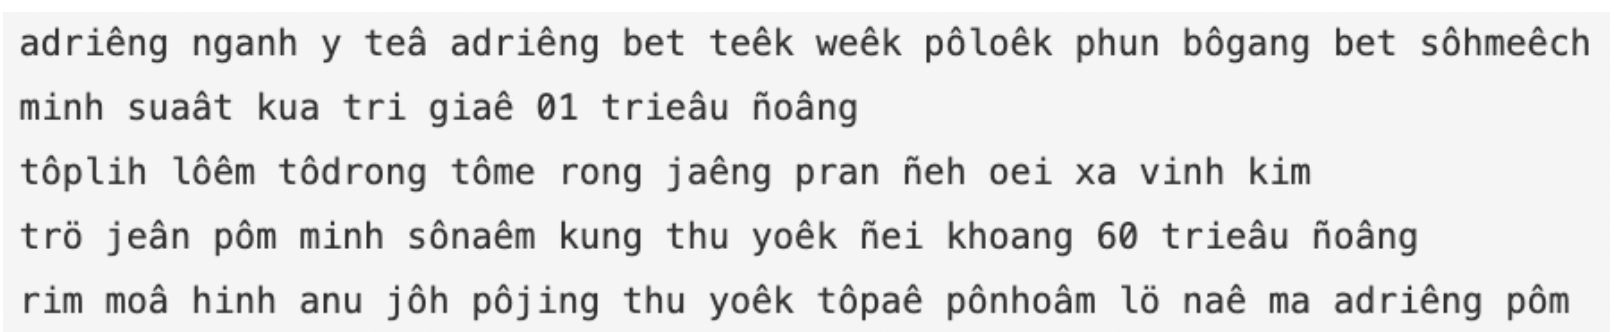
\includegraphics[scale=0.4]{image/bahna_example.png}
    \caption{Ví dụ về văn bản tiếng Bahnar}
\end{figure}
\pause
Một phân tích về tiếng Bahnar \cite{bahnarphenon} đã được tiến hành để tạo ra một tập hợp các âm vị phù hợp cho văn bản
\begin{itemize}
    \item Âm đơn: a, â, ĩ, ỉ, ợ, ữ ,.... 
    \item Nguyên âm đôi: ia, iă, iô, uê, ...
    \item Phụ âm kép: br, by, mr, ny, ...
    \item Phụ âm ba: ngl, ngy, phy, khy, ...
\end{itemize}
\end{frame}
\begin{frame}
\frametitle{Hệ thống ngữ âm tiếng Bahnar}
\begin{itemize}
    \item Tiếng Bahnar có bảng chữ cái, cấu tạo âm, vần khá giống tiếng Việt
    \item Tiếng Bahnar thường sử dụng từ mượn từ tiếng Việt cho những từ trong ngôn ngữ chưa có 
    \item[$\rightarrow$] Tiếng Bahnar và tiếng Việt có độ tương đồng với nhau
\end{itemize}
\end{frame}
\begin{frame}
\frametitle{Hệ thống ngữ âm tiếng Bahnar}
Bảng chữ cái âm vị dùng để so sánh từng từ trong văn bản đầu vào với chuỗi âm vị tương ứng của nó.
\begin{figure}
    \centering
    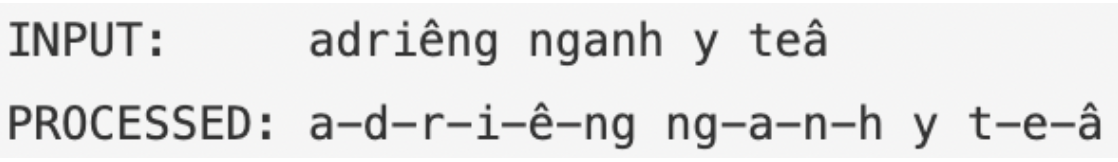
\includegraphics[scale=0.3]{image/bahna-processed.png}
    \caption{Ví dụ về xử lý đầu vào tiếng Bahnar}
\end{figure}
\end{frame}
%------------------------------------------------
%------------------------------------------------
\subsection{Mô hình tham khảo}
{
    \begin{frame}
        \frametitle{Mục lục}
        \tableofcontents[currentsection, currentsubsection]
    \end{frame}
}
\begin{frame}
\frametitle{Mô hình tham khảo}
Mô hình đề xuất được tham khảo và sử dụng lại các mô hình dưới đây
\begin{itemize}
    \item Mô hình Grad-TTS \footfullcite{gradtts}
    \item Mô hình HiFi-GAN \footfullcite{hifigan}
    \item Mô hình StarGANv2-VC \footfullcite{starganv2}
\end{itemize}
\end{frame}

%------------------------------------------------
%------------------------------------------------
% \begin{frame}
% \frametitle{Mô hình tham khảo StarGanV2}
% Tổng quan kiến trúc StarGANv2
% \begin{figure}
%     \centering
%     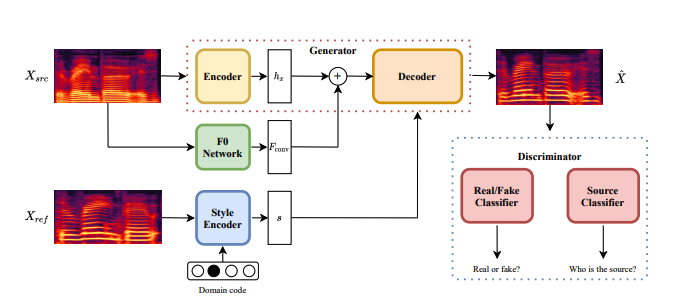
\includegraphics[scale=0.3]{image/starganv2.png}
%     \caption{Kiến trúc mô hình StarGANv2}
%     \label{fig:enter-label}
% \end{figure}
% \end{frame}

%------------------------------------------------
%------------------------------------------------
%------------------------------------------------

%------------------------------------------------
\subsection{Mô hình BN-TTS-VC}
{
    \begin{frame}
        \frametitle{Mục lục}
        \tableofcontents[currentsection, currentsubsection]
    \end{frame}
}
\begin{frame}
\frametitle{Mô hình BN-TTS-VC}
\begin{columns}[c] % The "c" option specifies centered vertical alignment while the "t" option is used for top vertical alignment

\column{.45\textwidth} % Left column and width
\begin{itemize}
    \item Hệ thống BN-TTS-VC bao gồm hai module chính, chuyển văn bản thành giọng (TTS) nói chuyển đổi giọng nói (VC)
    \item Trong module TTS, văn bản tiếng Bahnar là đầu vào để tạo ra giọng nói tương ứng với nội dung đầu vào
    \item Các dạng sóng âm thanh được tạo ra sẽ được chuyển đến module VC để tạo ra các loại giọng nói khác nhau dựa trên giọng nói tham chiếu.
\end{itemize}

\column{.5\textwidth} % Right column and width
\begin{figure}
    \centering
    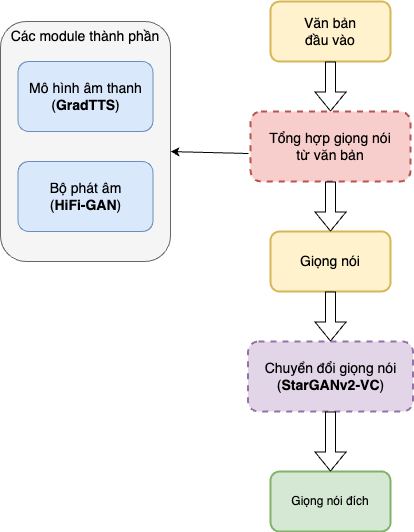
\includegraphics[scale=0.35]{image/proposed.drawio.png}
    \caption{Kiến trúc mô hình đề xuất}
\end{figure}

\end{columns}

\end{frame}
%------------------------------------------------
%------------------------------------------------
\begin{frame}
\frametitle{Mô hình Grad-TTS cho tiếng Bahnar}
\begin{itemize}
    \item [--] Ít nghiên cứu về tạo giọng nói nhân tạo cho ngôn ngữ dân tộc thiểu số.
    \item [--] Những đặc điểm độc đáo của tiếng Bahnar khiến việc áp dụng các kỹ thuật thông thường trở nên khó khăn.
    \item [--] Tiếng Việt và tiếng Bahnar có một sự tương đồng nhất định 
    \item [$\rightarrow$] Sử dụng kiến trúc Grad-TTS, mạng lưới thần kinh dựa trên mô hình xác suất khuếch tán khử nhiễu \cite{ddpm}, để tổng hợp giọng nói từ đầu đến cuối, phù hợp với các nghiên cứu liên quan ở các ngôn ngữ gần tiếng Bahnar, như tiếng Việt \footfullcite{tungpaper}.
\end{itemize}
\end{frame}
%------------------------------------------------
%------------------------------------------------
\begin{frame}
\frametitle{Mô hình Grad-TTS cho tiếng Bahnar}
Mô hình gồm các thành phần như sau:
\begin{itemize}
    \item Module phân tích văn bản: phân tích văn bản thành biểu diễn giả ngữ âm để xử lý mạng thần kinh.
    \item Mô hình âm thanh: dựa trên Grad-TTS lấy các âm vị giả làm đầu vào và tạo ra biểu diễn mel-spectrogram.
    \item Bộ mã hóa âm thanh: sử dụng mạng HiFi-GAN để chuyển đổi đầu ra mel-spectrogram thành dạng sóng giọng nói.
\end{itemize}
\begin{figure}
    \centering
    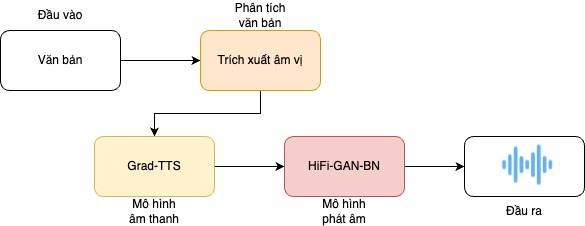
\includegraphics[scale=0.35]{image/tts-flow.jpeg}
    \caption{Quá trình xử lý của Grad-TTS cho tiếng Bahnar}
\end{figure}
\end{frame}
%------------------------------------------------
%------------------------------------------------

\begin{frame}
\frametitle{Mô hình HiFi-GAN cho tiếng Bahnar}
Thách thức nảy sinh khi áp dụng HiFi-GAN pre-train cho tiếng Anh sang tiếng Bahnar do sự khác biệt về ngôn ngữ và âm thanh.\\
$\rightarrow$ Để giải quyết vấn đề này, huấn luyện HiFi-GAN trên tập dữ liệu tiếng Bahnar
\pause
\begin{columns}[c] % The "c" option specifies centered vertical alignment while the "t" option is used for top vertical alignment

\column{.4\textwidth} % Left column and width
\begin{itemize}
    \item Mô hình huấn luyện bao gồm một bộ sinh và hai bộ phân biệt: bộ phân biệt đa giai đoạn và bộ phân biệt đa chu kỳ.
    \item Mô hình phát âm HiFi-GAN ở mô hình đề xuất sẽ áp dụng depth-wise separable convolution \cite{mobilenet} cho các lớp convolution 1D ở bộ sinh.
\end{itemize}

\column{.6\textwidth} % Right column and width
\begin{figure}
    \centering
    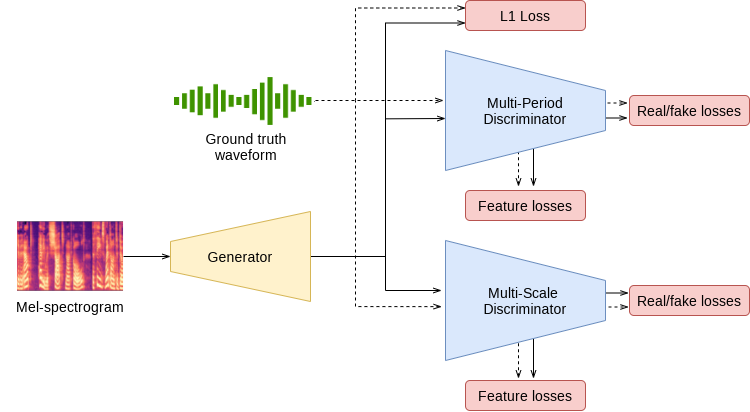
\includegraphics[scale=0.28]{image/hifigan_model.png}
    \caption{Mô hình HiFi-GAN \cite{hifigan}}
\end{figure}

\end{columns}
\end{frame}


%------------------------------------------------
%------------------------------------------------
\begin{frame}
\frametitle{Mô hình StarGANv2-VC cho tiếng Bahnar}
\begin{itemize}
    \item Grad-TTS có thể phát âm nhưng thiếu tự nhiên do ít dữ liệu cho tiếng Bahnar.\\
$\rightarrow$ Mô hình StarGANv2-VC dùng chuyển đổi giọng nói tổng hợp sang tiếng Bahnar bản địa.\\
\pause
    \item StarGANv2-VC tận dụng các nguyên tắc nền tảng của StarGANv2 \cite{star}, một mô hình tiên phong để tạo ra các hình ảnh đa dạng trên các miền. Trong chuyển đổi giọng nói, mỗi giọng đại diện cho một miền riêng biệt.\\
$\rightarrow$ Mục tiêu chính của StarGANv2-VC là thiết lập chức năng ánh xạ chuyển đổi đầu vào từ miền này sang miền khác mà không cần dựa vào dữ liệu song song.
\end{itemize}

\end{frame}
%------------------------------------------------
%------------------------------------------------
\begin{frame}
\frametitle{Mô hình StarGANv2-VC cho tiếng Bahnar}
\begin{columns}[c] % The "c" option specifies centered vertical alignment while the "t" option is used for top vertical alignment

\column{.42\textwidth} % Left column and width
Mô hình StarGANv2-VC gồm các thành phần:
\begin{itemize}
    \item Adversarial loss.
\item Adversarial source classifier loss.
\item Style reconstruction loss.
\item Style diversification loss.
\item F0 consistency loss.
\item Speech consistency loss.
\item Norm consistency loss.
\item Cycle consistency loss.
\end{itemize}

\column{.58\textwidth} % Right column and width
\begin{figure}
    \centering
    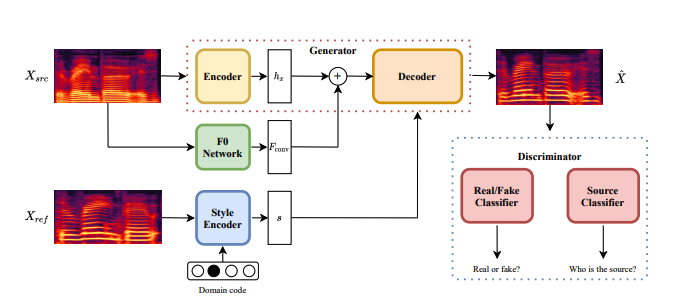
\includegraphics[scale=0.28]{image/starganv2.png}
    \caption{Kiến trúc mô hình StarGANv2-VC \cite{starganv2}}
\end{figure}
\end{columns}
\end{frame}

%------------------------------------------------
%------------------------------------------------
% \begin{frame}
% \frametitle{Mô hình StarGANv2-VC cho tiếng Bahnar}
% \begin{columns}[c] % The "c" option specifies centered vertical alignment while the "t" option is used for top vertical alignment

% \column{.4\textwidth} % Left column and width
% \begin{itemize}
%     \item Trong huấn luyện bộ phân biệt, trọng số của bộ tạo G vẫn cố định.
%     \item Bộ phân loại nguồn C được huấn luyện để xác định miền gốc $y_{k}$ của các mẫu được chuyển đổi, bỏ qua miền đích.
% \end{itemize}

% \column{.6\textwidth} % Right column and width
% \begin{figure}
%     \centering
%     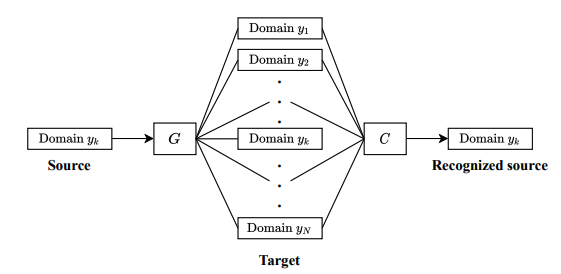
\includegraphics[scale=0.3]{image/starGAN-dis.png}
%     \caption{Mục tiêu huấn luyện bộ phân biệt \cite{starganv2}}
% \end{figure}

% \end{columns}

% \end{frame}
%------------------------------------------------
%------------------------------------------------
% \begin{frame}
% \frametitle{Mô hình StarGANv2-VC cho tiếng Bahnar}
% \begin{columns}[c] % The "c" option specifies centered vertical alignment while the "t" option is used for top vertical alignment

% \column{.4\textwidth} % Left column and width
% \begin{itemize}
%     \item Trong quá trình huấn luyện bộ sinh, trọng số của bộ phân loại nguồn C được giữ không đổi.
%     \item Bộ sinh G được huấn luyện để khiến C phân loại tất cả các mẫu được tạo như thể chúng có nguồn gốc từ miền đích $y_{k}$, bất kể miền nguồn thực tế.
% \end{itemize}

% \column{.6\textwidth} % Right column and width
% \begin{figure}
%     \centering
%     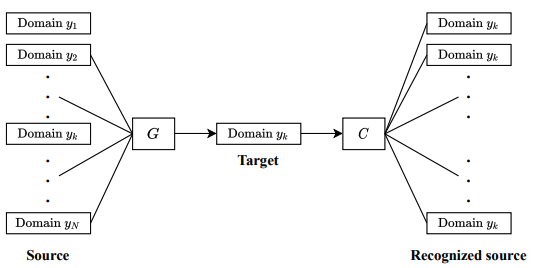
\includegraphics[scale=0.3]{image/starGAN-gen.png}
%     \caption{Mục tiêu huấn luyện bộ sinh \cite{starganv2}}
% \end{figure}

% \end{columns}

% \end{frame}
%------------------------------------------------

\section{Thí nghiệm và kết quả}
{
    \begin{frame}
        \frametitle{Mục lục}
        \tableofcontents[currentsection]
    \end{frame}
}% Sections can be created in order to organize your presentation into discrete blocks, all sections and subsections are automatically printed in the table of contents as an overview of the talk
%------------------------------------------------
\begin{frame}
\frametitle{Tập dữ liệu}
Mô hình đề xuất được huấn luyện trên tập dữ liệu bao gồm:
\begin{itemize}
    \item Dữ liệu tiếng Bahnar được thu âm ở Bình Định, Gia Lai và Kon Tum \footnote{by Ministry of Science and Technology (MOST) within the framework of the Program "Supporting research, development and technology application of Industry 4.0"KC-4.0/19-25 – Project “Development of a Vietnamese- Bahnaric machine translation and Bahnaric textto-speech system (all dialects)” - KC-4.0-29/19-25.}
    \item Dữ liệu tiếng Bahnar được thu thập từ trang Youtube VTV5 - Nhịp sống đồng bào \footnote{\href{https://www.youtube.com/@vtv5nhipsong}{VTV5 - Nhịp sống đồng bào}}
\end{itemize}
\end{frame}

%------------------------------------------------
\begin{frame}
\frametitle{Thí nghiệm và kết quả}
\begin{itemize}
    \item Mô hình HiFi-GAN được huấn luyện 100000 epoch trên G100 GPU với tập dữ liệu tiếng Bahnar thu thập từ Youtube
    \pause
    \item Mô hình Grad-TTS được huấn luyện 2500 epoch trên G100 GPU với tập dữ liệu thu âm từ Bình Định, Gia Lai và Kon Tum
    \pause 
    \item Mô hình StarGANv2-VC được huấn luyện 120 epoch trên G100 GPU với tập dữ liệu thu âm từ Bình Định, Gia Lai và Kon Tum
\end{itemize}
\end{frame}
%------------------------------------------------
%------------------------------------------------
\begin{frame}
\frametitle{Kết quả thí nghiệm}
Để đánh giá chất lương mô hình StarGANv2-VC, sử dụng mô hình AlexNet \cite{alexnet} để nhận dạng giọng nói
\begin{table}
\begin{tabular}{l l}
\toprule
\textbf{Version} & \textbf{Kết quả} \\
\midrule
Nam Bình Định & 90,12\% \\
Nữ Bình Định & 89,03\% \\
Nam Kon Tum & 83.77\% \\
Nữ Kon Tum & 86.55\% \\
Nam Gia Lai & 85.17\% \\
Nữ Gia Lai & 84.39\% \\
\bottomrule
\end{tabular}
\caption{Bảng kết quả StarGANv2-VC}
\end{table}
\end{frame}
%------------------------------------------------
\begin{frame}
\frametitle{Kết quả thí nghiệm}
Mô hình đề xuất BN-TTS-VC được đánh giá về chất lượng đầu ra bằng MOS có kết quả như sau
\begin{table}
\begin{tabular}{l l}
\toprule
\textbf{Version} & \textbf{MOS} \\
\midrule
Bản thu âm gốc & 4.50 \\
BN-TTS-VC & 4.02 \\
GradTTS-HiFiGan-origin & 3.51 \\
\bottomrule
\end{tabular}
\caption{Bảng kết quả MOS của mô hình đề xuất}
\end{table}
\end{frame}

%------------------------------------------------



%------------------------------------------------
%------------------------------------------------
\section{Kết luận}
{
    \begin{frame}
        \frametitle{Mục lục}
        \tableofcontents[currentsection]
    \end{frame}
}% Sections can be created in order to organize your presentation into discrete blocks, all sections and subsections are automatically printed in the table of contents as an overview of the talk
%------------------------------------------------
\begin{frame}
\frametitle{Kết quả đạt được}
\begin{itemize}
    \item [--] Xây dựng được mô hình chuyển văn bản thành giọng nói cho tiếng Bahnar
    \item [--] Thu thập và tiền xử lí bộ dữ liệu âm thanh từ Youtube 
    \item[--] Tìm hiểu được nội dung của bài toán tổng hợp giọng nói, cụ thể là Bài toán tổng hợp giọng nói từ văn bản, chuyển đổi giọng nói, các cơ sở lý thuyết, các công trình nghiên cứu liên quan và chỉ ra được ưu nhược điểm của chúng.
    \item[--] Xác định và nắm rõ mô hình cơ sở, chỉ ra ưu và nhược điểm của mô hình này. Đưa ra đề xuất cải tiến cùng động lực đi kèm.

\end{itemize}
\end{frame}

%------------------------------------------------
%------------------------------------------------
\begin{frame}
\frametitle{Những hạn chế và tồn đọng}
\begin{itemize}
    \item[--] Với mô hình đề xuất, vẫn còn một số mẫu âm thanh sinh ra có độ tự nhiên kém, không đạt yêu cầu khi thực hiện đánh giá 

    \item[--] Do hạn chế về thời gian thực hiện luận văn, các kết quả ghi nhận được mới chỉ dừng lại ở những thí nghiệm đơn giản và hàn lâm, chưa triển khai vào những hệ thống thực sự có thể có ích hơn như kết hợp với một mô hình dịch để có thể có một hệ thống dịch và phát âm từ tiếng Việt qua tiếng Bahnar.

    \item[--] Chưa đánh giá được về thời gian để sinh ra âm thanh từ văn bản ban đầu trên các phần cứng khác nhau.
    
\end{itemize}
\end{frame}

%------------------------------------------------
%------------------------------------------------
\begin{frame}
\frametitle{Hướng phát triển trong tương lai}
\begin{itemize}
    \item[--] Phân tích các mẫu âm thanh tạo ra kém, để có thể thu thập thêm dữ liệu về phát âm của từ để cải tiến thêm cho mô hình
    \item[--] Huấn luyện thêm mô hình Grad-TTS với tập dữ liệu chưa được huấn luyện
    \item[--] Xây dựng bộ phân tích từ vựng, và các bộ mạng F0 cho tiếng Bahnar để có thể đạt kết quả tốt hơn
    \item[--] Triển khai mô hình cho một hệ thống thực tế để theo dõi tính ổn định và hiệu quả của mô hình
\end{itemize}

\end{frame}

%------------------------------------------------
\begin{frame}
\frametitle{Demo video}
\begin{center}
    \href{https://youtu.be/ZkYbxshOVbU}{Demo video link}
\end{center}


\end{frame}

%------------------------------------------------

% \begin{frame}
% \frametitle{Bullet Points}
% \begin{itemize}
% \item Lorem ipsum dolor sit amet, consectetur adipiscing elit
% \item Aliquam blandit faucibus nisi, sit amet dapibus enim tempus eu
% \item Nulla commodo, erat quis gravida posuere, elit lacus lobortis est, quis porttitor odio mauris at libero
% \item Nam cursus est eget velit posuere pellentesque
% \item Vestibulum faucibus velit a augue condimentum quis convallis nulla gravida
% \end{itemize}
% \end{frame}

%------------------------------------------------

% \begin{frame}
% \frametitle{Blocks of Highlighted Text}
% \begin{block}{Block 1}
% Lorem ipsum dolor sit amet, consectetur adipiscing elit. Integer lectus nisl, ultricies in feugiat rutrum, porttitor sit amet augue. Aliquam ut tortor mauris. Sed volutpat ante purus, quis accumsan dolor.
% \end{block}

% \begin{block}{Block 2}
% Pellentesque sed tellus purus. Class aptent taciti sociosqu ad litora torquent per conubia nostra, per inceptos himenaeos. Vestibulum quis magna at risus dictum tempor eu vitae velit.
% \end{block}

% \begin{block}{Block 3}
% Suspendisse tincidunt sagittis gravida. Curabitur condimentum, enim sed venenatis rutrum, ipsum neque consectetur orci, sed blandit justo nisi ac lacus.
% \end{block}
% \end{frame}

%------------------------------------------------

% \begin{frame}
% \frametitle{Multiple Columns}
% \begin{columns}[c] % The "c" option specifies centered vertical alignment while the "t" option is used for top vertical alignment

% \column{.45\textwidth} % Left column and width
% \textbf{Heading}
% \begin{enumerate}
% \item Statement
% \item Explanation
% \item Example
% \end{enumerate}

% \column{.5\textwidth} % Right column and width
% Lorem ipsum dolor sit amet, consectetur adipiscing elit. Integer lectus nisl, ultricies in feugiat rutrum, porttitor sit amet augue. Aliquam ut tortor mauris. Sed volutpat ante purus, quis accumsan dolor.

% \end{columns}
% \end{frame}
%------------------------------------------------


% \begin{frame}
% \frametitle{Table}
% \begin{table}
% \begin{tabular}{l l l}
% \toprule
% \textbf{Treatments} & \textbf{Response 1} & \textbf{Response 2}\\
% \midrule
% Treatment 1 & 0.0003262 & 0.562 \\
% Treatment 2 & 0.0015681 & 0.910 \\
% Treatment 3 & 0.0009271 & 0.296 \\
% \bottomrule
% \end{tabular}
% \caption{Table caption}
% \end{table}
% \end{frame}

%------------------------------------------------

% \begin{frame}
% \frametitle{Theorem}
% \begin{theorem}[Mass--energy equivalence]
% $E = mc^2$
% \end{theorem}
% \end{frame}

%------------------------------------------------

% \begin{frame}[fragile] % Need to use the fragile option when verbatim is used in the slide
% \frametitle{Verbatim}
% \begin{example}[Theorem Slide Code]
% \begin{verbatim}
% \begin{frame}
% \frametitle{Theorem}
% \begin{theorem}[Mass--energy equivalence]
% $E = mc^2$
% \end{theorem}
% \end{frame}\end{verbatim}
% \end{example}
% \end{frame}


%------------------------------------------------

% \begin{frame}[fragile] % Need to use the fragile option when verbatim is used in the slide
% \frametitle{Citation}
% An example of the \verb|\cite| command to cite within the presentation:\\~

% This statement requires citation \cite{p1}.
% \end{frame}

%------------------------------------------------



%------------------------------------------------

\begin{frame}
\huge{\centerline{Xin cảm ơn quý thầy cô đã lắng nghe!}}
\end{frame}

%----------------------------------------------------------------------------------------
% \begin{frame}[allowframebreaks]
% \frametitle{Tài liệu tham khảo}
% \footnotesize{
% \begin{thebibliography}{99} % Beamer does not support BibTeX so references must be inserted manually as below
% \bibitem[Smith, 2012]{p1} John Smith (2012)
% \newblock Title of the publication
% \newblock \emph{Journal Name} 12(3), 45 -- 678.
% \end{thebibliography}
% }
% \end{frame}
\section{}
\begin{frame}[allowframebreaks]
\frametitle{Tài liệu tham khảo}
% \bibliography{rs_test}
\printbibliography

\end{frame}

\appendix

\begin{frame}
\frametitle{Phụ lục Tham số cấu hình}
Thông số thay đổi ở lớp convolution mô hình HiFi-GAN được thể hiện trong bảng dưới đây
\begin{table}
\begin{tabular}{l l l}
\toprule
\textbf{} & \textbf{Đề xuất} & \textbf{Mô hình gốc}\\
\midrule
Dialtion & [[1, 1], [3, 1], [5, 1]] & [1,3,5] \\
Parameters & 10.38M & 13.94M \\
\bottomrule
\end{tabular}
\caption{Thông số cho mô hình đề xuất}
\end{table}
\end{frame}

\end{document}